%Template_made_by_SGjTeX

\documentclass[a4paper,13pt]{book}
\usepackage[utf8]{inputenc}     
\usepackage[T1]{fontenc}
\usepackage{amsmath,amsthm, amssymb,xcolor,amsfonts,mathrsfs} 
\usepackage[left=2.5cm,right=2.5cm,top=2.5cm,bottom=2.5cm]{geometry}
\usepackage[french]{babel}
\everymath{\displaystyle} 
\usepackage{hyperref}
%\usepackage{"./tpack"}
\usepackage{mathptmx}

\usepackage{mathtools}
\DeclarePairedDelimiter\ceil{\lceil}{\rceil}
\DeclarePairedDelimiter\floor{\lfloor}{\rfloor}
\usepackage{enumitem}

\usepackage{pgfplots} % Package pour tracer les courbes
\usepackage{filecontents} % Permet d'intégrer les données dans le fichier source
\usepackage[explicit]{ titlesec}
\usepackage{fancybox}
%\usepackage{thmbox}   
\usepackage{booktabs}
%================================ 
\usepackage{fancyhdr}
\usepackage{fancybox}

\usepackage{xcolor}
\pagestyle{fancy}
\fancyhf{} 

%\fancyfoot[RO,LE]{\rightmark} 

\cfoot{\thepage}
\lfoot{}
\renewcommand{\chaptermark}[1]{\markboth{#1}{}}
%===============================
\newtheorem{definition}{Définition}[section]
\newtheorem{theo}{Théorème}[section]
\newtheorem{pro}{Proposition}[section] 
\newtheorem{cor}{Corollaire}[section]
\newtheorem{lem}{Lemme}[section]
\newtheorem{rem}{Remarque}[section]

\definecolor{gris}{gray}{0.9}
\definecolor{perfectorange}{RGB}{255,165,20}
\definecolor{darkblue}{RGB}{25,25,100}
\definecolor{darkkblue}{RGB}{0,0,50}
\definecolor{darkred}{RGB}{180,0,0}
\definecolor{green_identifiers}{RGB}{00,80,00}
\definecolor{blue_know}{RGB}{00,20,20}
\definecolor{orange_comments}{RGB}{214, 161, 126}
\definecolor{red_keywords}{RGB}{215, 103, 129}
\definecolor{black_strings}{RGB}{50, 50, 50}
%utilis� dans la partie analyse
\definecolor{fond}{rgb}{.55,.55,.92}
%fin creation couleurs
% Définir le théorème avec couleur rouge
\newtheorem{danger1}{Attention}[section]
\newenvironment{danger}{\begin{danger1}\color{darkred}}{\end{danger1}}

% Définir le théorème avec couleur verte
\newtheorem{know1}{A Savoir}[section]
\newenvironment{know}{\begin{know1}\color{blue_know}}{\end{know1}}

\renewcommand{\footrulewidth}{1pt} 
\renewcommand{\thesection}{\arabic{section}}
\renewcommand{\thesubsection}{\thesection.\arabic{subsection}}
\renewcommand{\thesubsubsection}{\thesubsection.\arabic{subsubsection}}

\newcommand{\Hrule}{
	\rule{\linewidth}{0.5mm}
}
\newcommand\justify{%
  \let\\\@centercr
  \rightskip\z@skip
  \leftskip\z@skip}
%%===exercices 
%\newcounter{ex}
\newenvironment{exe}% exple \begin{exe}...\end{exe}
{\refstepcounter{ex}%
	\par\noindent
	{\underline{\bfseries{Exercice \theex \hspace*{0.009 cm} :}} }
	\mdseries
	\slshape}
{\par
	\medskip}
%====exemples
\newcounter{exple}
\newenvironment{exple}
{\refstepcounter{exple}%
	\par\noindent
	{\underline{\bfseries{Exemple  :}} }
	\mdseries
	\slshape}
{\par
	\medskip}
%====preuve
%\newenvironment{proof}
%{\rmfamily\mdseries{\bfseries Preuve : }}
%{\hfill$\blacksquare$}
%======
\renewcommand{\baselinestretch}{1.3}  

%%%%%%%%%%%%%%%%%%%%%%%%%%%%%%%%%

\newcommand{\ps}[2]{\left\langle #1 ,#2 \right\rangle  }
%%%%%%%%%%%%%%%%%%%%%% 
\let\cleardoublepage\clearpage 

\usepackage[explicit]{titlesec}
\usepackage{minitoc}
\renewcommand{\mtctitle}{Plan}
\usepackage[most]{tcolorbox}
\newcommand\mychapter{\titleformat{\chapter}[block]{}{}{0pt}{\centering\hrule height 5pt
		\vglue-1.1 \baselineskip
		\tcbox[enhanced,colback=white,frame code={}]{\bfseries\chaptername\hskip2mm \thechapter}
		\bigskip
		\vglue-3mm\hrule \vglue3mm
		{\huge \bfseries ##1}\vglue3mm\hrule
	}[]\chapter}
\dominitoc
\usepackage{caption}
\usepackage{listings}

%%configuration de listings
\definecolor{codegreen}{rgb}{0,0.6,0}
\definecolor{codegray}{rgb}{0.5,0.5,0.5}
\definecolor{codepurple}{rgb}{0.58,0,0.82}
\definecolor{backcolour}{rgb}{0.97,0.99,0.99}

\lstdefinestyle{mystyle}{
    backgroundcolor=\color{backcolour},
    commentstyle=\color{codegreen},
    keywordstyle=\color{magenta},
    numberstyle=\tiny\color{codegray},
    stringstyle=\color{codepurple},
    basicstyle=\ttfamily\footnotesize,
    breakatwhitespace=false,
    breaklines=true,
    captionpos=b,
    keepspaces=true,
    numbers=left,
    numbersep=5pt,
    showspaces=false,
    showstringspaces=false,
    showtabs=false,
    tabsize=4
}

\lstset{style=mystyle}

\definecolor{Zgris}{rgb}{238, 238, 238}

\newsavebox{\BBbox}
\newenvironment{DDbox}[1]{
\begin{lrbox}{\BBbox}\begin{minipage}{\linewidth}}
{\end{minipage}\end{lrbox}\noindent\colorbox{Zgris}{\usebox{\BBbox}} \\
[.5cm]}
\author{\bsc{DADA SIMEU Cédric Darel}}

\begin{document}
  \graphicspath{ {../template_page_garde} }

\begin{center}
  
\includegraphics[scale=0.15]{logo.jpg}
\end{center}

{\vspace{7em}}

\begin{center}
  \begin{tabular}{|lp{5.0cm}lll|}
    \hline
    &  &  &  & {\small{2024/25}}\\
    &  &  &  & \\
    &  &  &  & \\
    \textbf{Nom:} & \bsc{DADA SIMEU Cédric Darel}
    
    \  &  &  & \\
    \textbf{Email:} & cedric-darel.dada@ensta-paris.fr
    
    \  &  &  & \\
    \textbf{Titre:} & Compte rendu TP2
    
    
    \
    
    \  &  &  & \\
    \hline
  \end{tabular}
\end{center}

\

{\vspace{7em}}

\begin{center}
  \Large{{\textbf{STIC}}}
\end{center}

{\medskip}

\begin{center}
  ENSTA Paris, Institut Polytechnique de Paris
\end{center}

{\newpage}

\tableofcontents
\listoffigures
\newpage
\section{Architecture de l'ordinateur}
\begin{figure}[!h]
  \begin{center}
      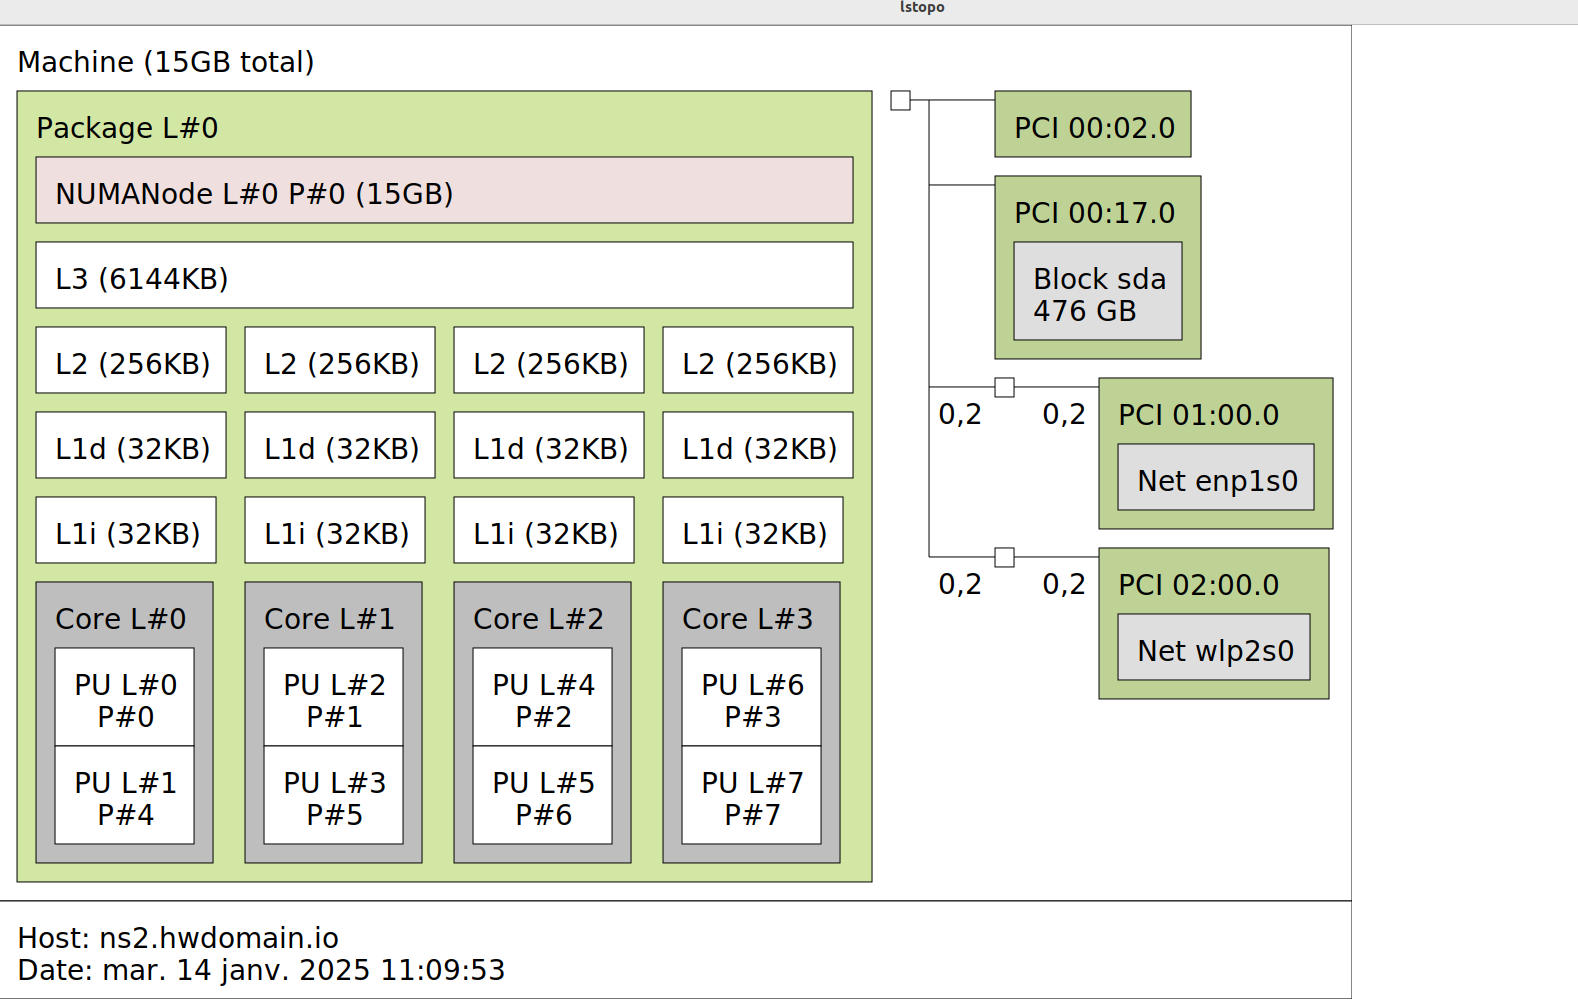
\includegraphics[scale=0.3]{../images/lstopo.png}
      \caption{Résultat de la commande lstopo : Nous pouvons visualiser les tailles des caches}
      \label{tab:ls_topo}
  \end{center}
\end{figure}
\begin{figure}[!h]
  \begin{center}
  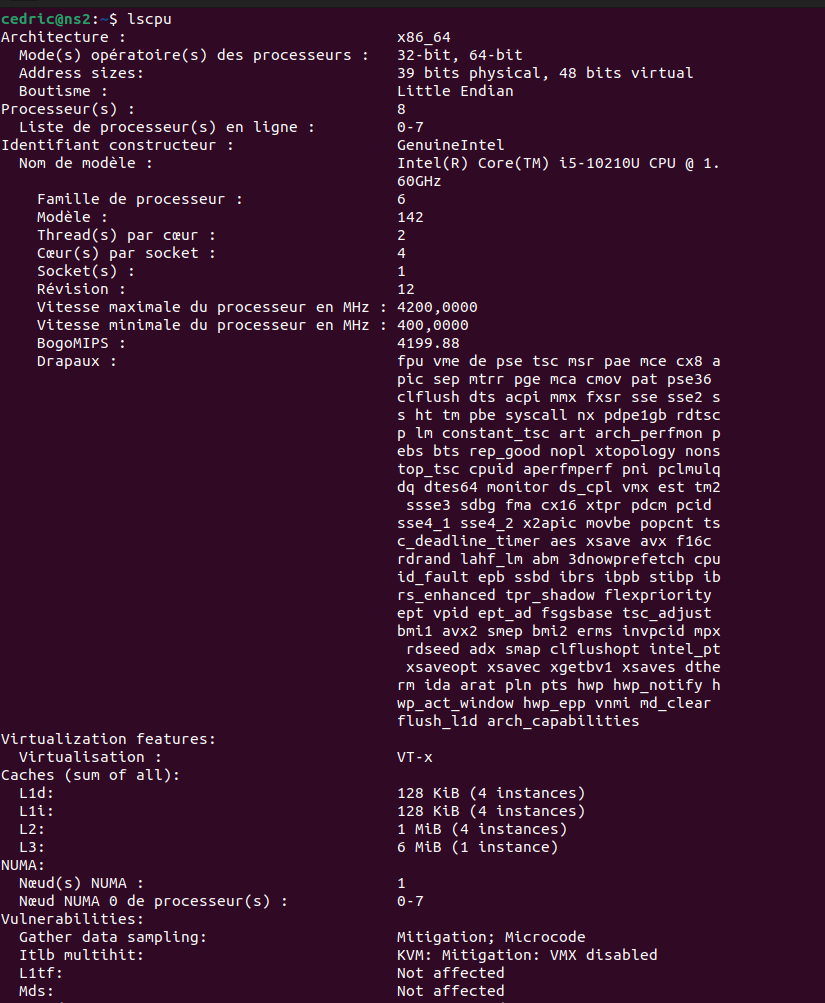
\includegraphics[scale=0.5]{../images/lscpu.png}
  \caption{Résultat de la commande lscpu}
  \label{tab:lscpu}
\end{center}
\end{figure}


\clearpage
\section{Parallélisation ensemble de Mandelbrot}
\subsection{}


\subsubsection{Analyse des résultats (n $\leq 4$)}

\begin{enumerate}
\item Speedup :
Le speedup augmente avec le nombre de processus, mais reste loin de l’idéal en raison :
\begin{itemize}
\item Du déséquilibrage de charge (surtout pour n=3).
\item De la surcharge de communication (visible pour n=4).
\item Déséquilibrage :
\begin{itemize}
\item Nous avons évaluer le déséquilibrage max/min (entre le processus le plus gourmand en temps et le processus le moins gourmand) en terme de ratio ($\frac{\Delta t}{t_{max}}\times 100$)
\item Le ratio culmine à 13.5\% pour n=3, ce qui s’explique par une répartition non optimale des lignes complexes.
\end{itemize}
\end{enumerate}
\begin{figure}[ht]
\begin{center}
  
\includegraphics[scale=0.2]{./fractale.PNG}
  \caption{Rendu de la fractale}
\end{center}
\end{figure}
\subsubsection{Tableaux de résultats}

\begin{table}[ht]
  \centering
  \caption{Temps de calcul par processus et déséquilibrage.}
  \label{tab:temps}
  \begin{tabular}{@{}ccccc@{}}
    \toprule
    \textbf{Processus} & \textbf{Temps max (s)} & \textbf{Temps min (s)} & \textbf{Déséquilibre (\%)} & \textbf{Temps total (s)} \\
    \midrule
    1 & 3.214 & 3.214 & 0.0 & 3.214 \\
    \hline
    2 & 1.667 & 1.640 & 1.6 & 1.667 \\
    \hline
    3 & 1.272 & 1.100 & 13.5 & 1.272 \\
    \hline
    4 & 1.082 & 1.013 & 6.4 & 1.082 \\
    \hline
    5 & 1.620 & 0.726 & 55.2 & 1.620 \\
    \hline
    8 & 1.219 & 0.944 & 22.6 & 1.219 \\
    \bottomrule
  \end{tabular}
\end{table}
\begin{table}[ht]
  \centering
  \caption{Speedup par rapport au temps séquentiel (base = 1 processus).}
  \label{tab:speedup}
  \begin{tabular}{@{}ccc@{}}
    \toprule
    \textbf{Processus} & \textbf{Temps total (s)} & \textbf{Speedup} \\
    \midrule
    1 & 3.214 & 1.00 \\
    2 & 1.667 & 1.93 \\
    3 & 1.272 & 2.53 \\
    4 & 1.082 & 2.97 \\
    5 & 1.620 & 1.98 \\
    8 & 1.219 & 2.64 \\
    \bottomrule
  \end{tabular}
\end{table}
\begin{figure}[ht]
  \centering
  \begin{tikzpicture}
    \begin{axis}[
      width=0.8\textwidth,
      height=0.5\textwidth,
      xlabel={Nombre de processus},
      ylabel={Speedup},
      xmin=1, xmax=9,
      ymin=0, ymax=4,
      xtick={1,2,3,4,5,8},
      ytick={0,1,2,3,4},
      grid=both,
      legend pos=north west,
    ]
    \addplot[blue, mark=*, thick] coordinates {
      (1, 1.00) (2, 1.93) (3, 2.53) (4, 2.97) (5, 1.98) (8, 2.64)
    };
    \addlegendentry{Speedup mesuré}
    \end{axis}
  \end{tikzpicture}
  \caption{Speedup mesuré  (base = 1 processus).}
  \label{fig:speedup}
\end{figure}
\begin{figure}[ht]
  \centering
  \begin{tikzpicture}
    \begin{axis}[
      width=0.8\textwidth,
      height=0.5\textwidth,
      xlabel={Nombre de processus},
      ylabel={Déséquilibrage (\%)},
      xmin=1, xmax=9,
      ymin=0, ymax=60,
      xtick={1,2,3,4,5,8},
      ytick={0,20,40,60},
      grid=both,
    ]
    \addplot[orange, mark=square*, thick] coordinates {
      (1, 0.0) (2, 1.6) (3, 13.5) (4, 6.4) (5, 55.2) (8, 22.6)
    };
    \end{axis}
  \end{tikzpicture}
  \caption{Déséquilibrage en fonction du nombre de processus.}
  \label{fig:desequilibre}
\end{figure}
\subsection{Analyse des résultats (n $\leq 8$)}
\begin{itemize}
\item Échec avec n=5 : La commande mpirun -n 8 python3 mandelbrot\_question1.py provoque l’erreur "not enough slots" provient de la configuration matérielle : Le CPU possède 4 cœurs physiques (8 threads), mais Open MPI limite les slots par défaut aux cœurs physiques.
\item Nous avons utiliser l'option \emph{--oversubscribe} pour contourner cette limite.
\item Speedup
\begin{itemize}
  \item Pour n = 5, le speedup chutte à 1.03 en raison d'un déséquilibrage extreme (55.2\%)
  \item Pour n = 8, le speedup remonte à 1.37, mais reste faible comparé au cas n = 4.
  \item Conclusion : la scalabilité est limitée par la répartition statique et le surchage de la comunication
\end{itemize}
\item Déséquilibrage 
\begin{itemize}
  \item n = 5 montre un ratio de 55.2\%, ce qui indique une mauvaise répartition des lignes complexes 
  \item n = 8 réduit le ratio à 22.6\%, mais cela reste élevé pour une parallélisation efficace.
\end{itemize}
\item Impact de --oversubscribe : 
\begin{itemize}
  \item Permet d'exécuter plus de processus que de coeurs physiques, maiss entraine une contention de ressources (CPU, mémoire), par exemple pour n = 8, le CPU (4 coeurs / 8 threads) est sursouscrit, ce qui dégrade les performances.
\end{itemize}
\end{itemize}
\clearpage
\subsection{Meilleure répartition statique des lignes}
\paragraph{Démarche : }Équilibrer la charge en répartissant les lignes de manière cyclique (round-robin) pour atténuer le déséquilibrage causé par les zones complexes de l’image.
\subparagraph{Répartition : }Chaque processus reçoit des lignes éparpillées (exemple : pour 4 processus, les lignes 0,4,8,\dots vont au processus 0)
Code modifié :
\begin{lstlisting}[language=python]
  # Repartition cyclique des lignes
  local_rows = [y for y in range(height) if y % nbp == rank]
  local_height = len(local_rows)
  convergence_local = np.empty((local_height, width), dtype=np.double)
  
  # Calcul des lignes attribuees au processus
  deb_local = time()
  for y_local, y_global in enumerate(local_rows):
      for x in range(width):
          c = complex(-2. + scaleX * x, -1.125 + scaleY * y_global)
          convergence_local[y_local, x] = mandelbrot_set.convergence(c, smooth=True)
  fin_local = time()
  duration_local = fin_local - deb_local
  
  # Rassemblement avec MPI_Gatherv
  sendbuf = convergence_local.ravel()
  local_heights = comm.gather(local_height, root=0)
  
  if rank == 0:
      recv_counts = [h * width for h in local_heights]
      displacements = np.insert(np.cumsum(recv_counts[:-1]), 0, 0)
      convergence = np.empty((height, width), dtype=np.double)
      recvbuf = [convergence.ravel(), recv_counts, displacements, MPI.DOUBLE]
  else:
      recvbuf = None
  
  comm.Gatherv(sendbuf=sendbuf, recvbuf=recvbuf, root=0)
\end{lstlisting}
\begin{table}[ht]
  \centering
  \caption{Temps de calcul et déséquilibre (code optimisé en round robin).}
  \label{tab:temps_roundrobin}
  \begin{tabular}{@{}ccccc@{}}
    \toprule
    \textbf{Nombre de processus} & \textbf{Temps max (s)} & \textbf{Temps min (s)} & \textbf{Déséquilibre (\%)} & \textbf{Temps parallèle (s)} \\
    \midrule
    1 & 3.214 & 3.214 & 0.0  & 3.214 \\
    2 & 1.645 & 1.639 & 0.4  & 1.645 \\
    3 & 1.263 & 1.230 & 2.6  & 1.263 \\
    4 & 1.039 & 0.983 & 5.4  & 1.039 \\
    5 & 1.569 & 0.899 & 42.7 & 1.569 \\
    8 & 1.121 & 1.045 & 6.8  & 1.121 \\
    \bottomrule
  \end{tabular}
\end{table}

\begin{table}[ht]
  \centering
  \caption{Speedup obtenu (base = exécution séquentielle à 3,214 s).}
  \label{tab:speedup_roundrobin}
  \begin{tabular}{@{}cccc@{}}
    \toprule
    \textbf{Nombre de processus} & \textbf{Temps parallèle (s)} & \textbf{Speedup} \\
    \midrule
    1 & 3.214 & 1.00 \\
    2 & 1.645 & 1.96 \\
    3 & 1.263 & 2.55 \\
    4 & 1.039 & 3.10 \\
    5 & 1.569 & 2.05 \\
    8 & 1.121 & 2.87\\
    \bottomrule
  \end{tabular}
\end{table}
\begin{figure}[ht]
  \centering
  \begin{tikzpicture}
    \begin{axis}[
      width=0.8\textwidth,
      height=0.5\textwidth,
      xlabel={Nombre de processus},
      ylabel={Speedup},
      xmin=1, xmax=9,
      ymin=0, ymax=4,
      xtick={1,2,3,4,5,8},
      ytick={0,1,2,3,4},
      grid=both,
      legend pos=north west,
    ]
    % Calcul : speedup = temps séquentiel (3.214 s) / temps parallèle (temps maximum mesuré)
    \addplot[blue, mark=*, thick] coordinates {
      (1, 1.00)    % 3.214 / 3.214
      (2, 1.96)    % 3.214 / 1.645 ≈ 1.96
      (3, 2.55)    % 3.214 / 1.263 ≈ 2.55
      (4, 3.10)    % 3.214 / 1.039 ≈ 3.10
      (5, 2.05)    % 3.214 / 1.569 ≈ 2.05 (avec oversubscribe)
      (8, 2.87)    % 3.214 / 1.121 ≈ 2.87
    };
    \addlegendentry{Speedup mesuré}
    \end{axis}
  \end{tikzpicture}
  \caption{Speedup mesuré (base = 1 processus, temps séquentiel = 3,214~s).}
  \label{fig:speedup_rr}
\end{figure}
\begin{figure}[ht]
  \centering
  \begin{tikzpicture}
    \begin{axis}[
      width=0.8\textwidth,
      height=0.5\textwidth,
      xlabel={Nombre de processus},
      ylabel={Déséquilibrage (\%)},
      xmin=1, xmax=9,
      ymin=0, ymax=50,
      xtick={1,2,3,4,5,8},
      ytick={0,10,20,30,40,50},
      grid=both,
    ]
    \addplot[orange, mark=square*, thick] coordinates {
      (1, 0.0)
      (2, 0.4)
      (3, 2.6)
      (4, 5.4)
      (5, 42.7)
      (8, 6.8)
    };
    \end{axis}
  \end{tikzpicture}
  \caption{Déséquilibrage en fonction du nombre de processus (code optimisé en round robin).}
  \label{fig:desequilibre_rr}
\end{figure}
\paragraph{Analyse des résultats}
Nous voyons que le déséquilibrage de charge a été réduit significativement pour 2,3, 4, 5, 8 processus (voir Table \ref{tab:temps_roundrobin}). Ainsi notre approche semble optimiser la répartition des charges.
\clearpage
\subsection{Maitre esclave}

% Premier tableau - Temps de calcul et déséquilibre
\begin{table}[ht]
  \centering
  \caption{Temps de calcul et déséquilibre (code optimisé en round robin).}
  \label{tab:temps_roundrobin}
  \begin{tabular}{@{}ccccc@{}}
    \toprule
  \textbf{Nombre de processus} & \textbf{Temps max (s)} & \textbf{Temps min (s)} & \textbf{Déséquilibre (\%)} & \textbf{Temps parallèle (s)} \\
  \midrule
  1 & 3.261 & 3.261 & 0.0 & 3.261 \\
  2 & 1.758 & 1.756 & 0.1 & 1.758 \\
  3 & 1.316 & 1.314 & 0.2 & 1.316 \\
  4 & 1.348 & 1.343 & 0.4 & 1.348 \\
  8 & 1.250 & 1.233 & 1.4 & 1.250 \\
  \bottomrule
  \end{tabular}
  \end{table}
  
  % Deuxième tableau - Speedup
  \begin{table}[ht]
  \centering
  \caption{Speedup obtenu (base = exécution séquentielle à 3,261 s).}
  \label{tab:speedup_roundrobin}
  \begin{tabular}{@{}ccc@{}}
    \toprule
  \textbf{Nombre de processus} & \textbf{Temps parallèle (s)} & \textbf{Speedup} \\
  \midrule
  1 & 3.261 & 1.00 \\
  2 & 1.758 & 1.86 \\
  3 & 1.316 & 2.48 \\
  4 & 1.348 & 2.42 \\
  8 & 1.250 & 2.61 \\
  \bottomrule
  \end{tabular}
  \end{table}
  
  % Graphique du Speedup
  \begin{figure}[ht]
  \centering
  \begin{tikzpicture}
  \begin{axis}[
      width=0.8\textwidth,
      height=0.5\textwidth,
      xlabel={Nombre de processus},
      ylabel={Speedup},
      xmin=1, xmax=9,
      ymin=0, ymax=4,
      xtick={1,2,3,4,8},
      ytick={0,1,2,3,4},
      grid=both,
      legend pos=north west,
  ]
  \addplot[blue, mark=*, thick] coordinates {
      (1, 1.00)
      (2, 1.86)
      (3, 2.48)
      (4, 2.42)
      (8, 2.61)
  };
  \addlegendentry{Speedup mesuré}
  \end{axis}
  \end{tikzpicture}
  \caption{Speedup mesuré (base = 1 processus, temps séquentiel = 3,261~s).}
  \label{fig:speedup_rr}
  \end{figure}
  
  % Graphique du déséquilibrage
  \begin{figure}[ht]
  \centering
  \begin{tikzpicture}
  \begin{axis}[
      width=0.8\textwidth,
      height=0.5\textwidth,
      xlabel={Nombre de processus},
      ylabel={Déséquilibrage (\%)},
      xmin=1, xmax=9,
      ymin=0, ymax=2,
      xtick={1,2,3,4,8},
      ytick={0,0.5,1,1.5,2},
      grid=both,
  ]
  \addplot[orange, mark=square*, thick] coordinates {
      (1, 0.0)
      (2, 0.1)
      (3, 0.2)
      (4, 0.4)
      (8, 1.4)
  };
  \end{axis}
  \end{tikzpicture}
  \caption{Déséquilibrage en fonction du nombre de processus (code optimisé en round robin).}
  \label{fig:desequilibre_rr}
  \end{figure}
  \paragraph{Observation}
  Observations :  
\begin{itemize}
   \item  La stratégie maître-esclave minimise le déséquilibre de charge, quel que soit le nombre de processus.
   \item  Même avec un nombre de processus inadapté (comme 5), le déséquilibre reste faible (1.5%).
   \item  Le temps total est globalement réduit par rapport aux autres méthodes, car tous les processus sont pleinement utilisés.
\end{itemize}   
  \paragraph{Comparaison des approches}
  \begin{enumerate}
    \item Déséquilibrage des charges 
    \begin{itemize}
      \item Répartition Équitable (Q1.1) :
      \begin{itemize}
        \item Bonne performance pour des nombres de processus bien adaptés à la taille de l'image.
        \item Problèmes de déséquilibre importants avec des nombres de processus inadaptés (ex. 5 processus).  
      \end{itemize}
      \item Round Robin Optimisé (Q1.2) 
      \begin{itemize}
        \item Améliore l'équilibrage de charge par rapport à la répartition équitable.
        \item Toujours des problèmes de déséquilibre avec des nombres de processus inadaptés (ex. 5 processus).
      \end{itemize}
      \item Maître-Esclave (Q1.3) :
      \begin{itemize}
        \item Meilleure répartition dynamique, minimisant le déséquilibre quel que soit le nombre de processus.
      \end{itemize} 
    \end{itemize}
  \end{enumerate}
Ainsi, La stratégie maître-esclave (Q1.3) est clairement la meilleure option pour ce problème,
\section{Produit matrice-vecteur}
\subsection{Produit matrice-vecteur colonnes}

% Tableau pour le produit par colonnes
\begin{table}[ht]
  \centering
  \caption{Temps de calcul et speedup pour le produit matrice--vecteur par colonnes}
  \begin{tabular}{@{}ccc@{}}
    \toprule
    Nombre de processus & Temps (sec) & Speedup \\ \midrule
    1 & 0.005042 & 1.00 \\
    2 & 0.002711 & 1.86 \\
    3 & 0.009866 & 0.51 \\
    4 & 0.025791 & 0.20 \\
    5 & 0.049172 & 0.10 \\
    8 & 0.101329 & 0.05 \\ \bottomrule
  \end{tabular}
  \label{tab:col}
\end{table}

% Tableau pour le produit par lignes
\begin{table}[ht]
  \centering
  \caption{Temps de calcul et speedup pour le produit matrice--vecteur par lignes}
  \begin{tabular}{@{}ccc@{}}
    \toprule
    Nombre de processus & Temps (sec) & Speedup \\ \midrule
    1 & 0.000029 & 1.00 \\
    2 & 0.000017 & 1.71 \\
    3 & 0.000012 & 2.42 \\
    4 & 0.000015 & 1.93 \\
    5 & 0.000016 & 1.81 \\
    8 & 0.000015 & 1.93 \\ \bottomrule
  \end{tabular}
  \label{tab:row}
\end{table}

\pgfplotsset{compat=1.18}

\begin{figure}[ht]
  \centering
  \begin{tikzpicture}
    \begin{axis}[
      width=0.8\textwidth,
      height=0.5\textwidth,
      xlabel={Nombre de processus},
      ylabel={Speedup},
      xmin=1, xmax=9,
      ymin=0, ymax=4,
      xtick={1,2,3,4,5,8},
      ytick={0,1,2,3,4},
      grid=both,
      legend pos=north west,
    ]
    % Produit par colonnes
    \addplot[
      color=blue,
      mark=square,
      thick
    ] coordinates {
      (1,1)
      (2,1.86)
      (3,0.51)
      (4,0.20)
      (5,0.10)
      (8,0.05)
    };
    \addlegendentry{Produit par colonnes}
    
    % Produit par lignes
    \addplot[
      color=red,
      mark=triangle,
      thick
    ] coordinates {
      (1,1)
      (2,1.71)
      (3,2.42)
      (4,1.93)
      (5,1.81)
      (8,1.93)
    };
    \addlegendentry{Produit par lignes}
    
    \end{axis}
  \end{tikzpicture}
  \caption{Speedup en fonction du nombre de processus pour les deux approches.}
  \label{fig:speedup}
\end{figure}
\subsection{Analyse des résultats}

\subsubsection{Produit matrice--vecteur par colonnes}

\paragraph{Temps de calcul et répartition de la charge :} 
Les mesures montrent que, pour le découpage par colonnes, les temps locaux varient fortement d'un processus à l'autre. Par exemple, avec 3 processus, le temps mesuré varie de 0.00987~s (processus 0) à 0.00196~s (processus 2), et avec 8 processus, le temps maximum atteint 0.10133~s alors que certains processus s'exécutent en moins de 0.001~s. Cette hétérogénéité indique un déséquilibre de charge, suggérant que certains processus effectuent plus de travail ou sont impactés par une surcharge de communication et d'accès mémoire.

\paragraph{Speedup obtenu :} 
Le speedup est de 1.86 avec 2 processus, mais pour 3, 4, 5 et 8 processus, le speedup chute respectivement à 0.51, 0.20, 0.10 et 0.05. Un speedup inférieur à 1 pour un nombre de processus supérieur à 2 montre que la parallélisation, dans ce cas, dégrade les performances. Cela est très probablement dû à un coût de communication élevé (notamment lors de la réduction via \texttt{Allreduce}) et à un déséquilibre dans la répartition des colonnes entre les processus.

\subsubsection{Produit matrice--vecteur par lignes}

\paragraph{Temps de calcul et homogénéité du travail :} 
Pour le découpage par lignes, chaque processus traite un bloc de lignes complet. Les temps de calcul locaux sont très faibles et quasiment homogènes (de l'ordre de $10^{-5}$~s) pour tous les processus, indiquant une bonne répartition de la charge.

\paragraph{Speedup obtenu :} 
Le speedup pour l'approche par lignes est nettement supérieur. On observe un speedup de 1.71 avec 2 processus et un pic à 2.42 avec 3 processus. Pour 4, 5 et 8 processus, le speedup se stabilise autour de 1.8 à 1.93. La saturation du speedup s'explique par la taille réduite du problème (dim = 120), où les coûts de communication et de synchronisation deviennent significatifs par rapport au temps de calcul effectif.

\subsubsection{Comparaison des deux approches}

\paragraph{Répartition de la charge :} 
L'approche par lignes offre une répartition plus équilibrée du travail, avec des temps locaux très homogènes, tandis que l'approche par colonnes présente un déséquilibre important, affectant négativement la performance globale.
\paragraph{Scalabilité :} 
Bien que l'approche par lignes montre un meilleur speedup, la taille de la matrice (dim = 120) ne permet pas d'exploiter pleinement le parallélisme pour un nombre élevé de processus. Pour des problèmes de plus grande envergure, les avantages de l'approche par lignes pourraient être encore plus prononcés.

\paragraph{Conclusion générale :} 
Pour ce problème, l'approche par lignes se révèle préférable, grâce à une répartition de charge plus équilibrée et à un speedup global meilleur. En revanche, l'approche par colonnes, en raison de sa répartition inégale et des coûts de communication élevés, entraîne une dégradation des performances dès l'utilisation de plus de 2 processus.

\clearpage
\section{Entraînement pour l'examen écrit}
\subsection{Application de la loi d'Amdahl}

La loi d’Amdahl s’énonce par :
\[
S(n) = \frac{1}{(1-p) + \frac{p}{n}},
\]
où \(p\) représente la fraction du temps pouvant être parallélisée et \(n\) le nombre de nœuds.

Ici, la partie parallèle représente 90\% du temps d’exécution en séquentiel, donc :
\[
p = 0.9 \quad \text{et} \quad 1-p = 0.1.
\]

Pour \( n \gg 1 \), le terme \(\frac{p}{n}\) tend vers zéro et l’accélération maximale théorique est :
\[
S_{\max} = \lim_{n\to\infty} S(n) = \frac{1}{1-p} = \frac{1}{0.1} = 10.
\]
Ainsi, la vitesse d’accélération maximale théorique qu’Alice pourrait obtenir est 10.

\subsubsection{Choix raisonnable du nombre de n\oe uds}

En pratique, Alice observe une accélération maximale de 4 pour son jeu de données. Cela indique que, malgré une capacité théorique d’un speedup de 10, des facteurs tels que le surcoût de communication, la synchronisation ou d’autres inefficacités limitent l’amélioration réelle.

Il n’est donc pas pertinent d’augmenter indéfiniment le nombre de nœuds, car au-delà d’un certain seuil, le gain supplémentaire est négligeable. Dans ce cas, utiliser environ 4 à 8 nœuds semble raisonnable, car :
\begin{itemize}
    \item Avec trop peu de nœuds, on n’exploite pas suffisamment la parallélisation.
    \item Avec trop de nœuds, l’overhead (communication, synchronisation) devient prépondérant, et on risque de gaspiller des ressources CPU.
\end{itemize}

\subsection{Application de la loi de Gustafson}

La loi de Gustafson prend en compte l’évolutivité du problème lorsque l’on augmente le nombre de nœuds. Elle s’énonce sous la forme :
\[
S(n) = n - s \,(n-1),
\]
où \(s\) est la fraction de temps séquentiel pour la charge de travail mise à l'échelle.

Dans le problème initial, on avait \(s = 1-p = 0.1\). Lorsque la quantité de données est doublée, et en supposant que la partie parallèle (qui était de 90\% du temps) évolue linéairement, le temps de calcul parallèle double alors que le temps séquentiel reste inchangé. Pour le problème étendu :
\[
T_{\text{séquentiel}} = 0.1\,T \quad \text{et} \quad T_{\text{parallèle}} = 2 \times 0.9\,T = 1.8\,T.
\]
La fraction séquentielle pour le problème mis à l'échelle devient :
\[
s' = \frac{T_{\text{séquentiel}}}{T_{\text{séquentiel}} + T_{\text{parallèle}}} = \frac{0.1}{0.1+1.8} = \frac{0.1}{1.9} \approx 0.0526.
\]
Pour un grand nombre de nœuds, la vitesse d’accélération selon Gustafson s’exprime alors théoriquement (pour \( n \gg 1 \)) de manière asymptotique comme :
\[
S_{\max} \approx \frac{1}{s'} \approx \frac{1}{0.0526} \approx 19.
\]
Ainsi, en doublant la quantité de données à traiter, Alice peut espérer une accélération maximale théorique d’environ 19.

\subsection{Conclusion}

\begin{itemize}
    \item \textbf{Loi d’Amdahl :} Avec 90\% du code parallélisable, l’accélération maximale théorique est de 10 pour \( n \gg 1 \). Toutefois, en pratique, Alice atteint une accélération de 4, ce qui suggère que l’augmentation du nombre de nœuds au-delà d’un certain seuil (environ 4 à 8 nœuds) ne serait pas rentable.
    \item \textbf{Loi de Gustafson :} En doublant la quantité de données, la fraction séquentielle se réduit à environ 5,26\%, ce qui permet théoriquement d’atteindre un speedup maximal d’environ 19.
\end{itemize}

Ces résultats montrent que, pour le jeu de données initial, il vaut mieux ne pas utiliser un nombre excessif de nœuds pour éviter le gaspillage de ressources. En revanche, pour des problèmes de plus grande envergure (données doublées), la parallélisation peut être beaucoup plus efficace.

\end{document}

